\begin{XeClass}{BufferedFSInputStream}
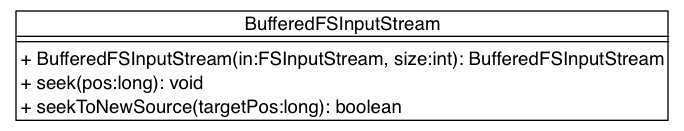
\includegraphics[width=\textwidth]{cdig/BufferedFSInputStream.png}
     
 BufferedFSInputStream继承了\emph{BufferedInputStream},
 通过缓存来优化其内包装的对象\emph{FSInputStream}的读取

    \begin{XeMethod}{\XePublic}{BufferedFSInputStream}{BufferedFSInputStream}
         
 创建一个指定buffer大小为size的\emph{BufferedFSInputStream}

    \end{XeMethod}

    \begin{XeMethod}{\XePublic}{void}{seek}
         
 如果要移动到的目标读取位置在目前的buffer中,那么优化他,直接在
 buffer内移动读取位置。

    \end{XeMethod}

    \begin{XeMethod}{\XePublic}{boolean}{seekToNewSource}
         
 将输入源切换到一个新的输入源,并且将偏移量移动到\emph{pos}。
 此方法在FTP、S3、Local等文件系统上均无实现(直接返回false),现有
 的唯一实现在\emph{org.apache.hadoop.hdfs.DFSInputStream.seekToNewSource(long targetPos)},其功能是在当前读取的Block失效时,切换到新的Block,并且移动偏移量,操作成
 功时返回true

    \end{XeMethod}

\end{XeClass}
